\documentclass{article}
\usepackage{amsmath}
\usepackage{float}

\usepackage{graphicx} 
\graphicspath{ {./images/} }

\title{CA Project Report}
\author{
    Abdelrahman Elsamalouty(55-0842) T-21\\
    \\
    Abdelrahman Elaby(55-0990) T-21 \\
    \\
    Habiba Hesham(55-0966) T-21\\
    \\
    Hazem Mansour(55-1036) T-21\\
    \\
    Zeina Mohamed(55-1095) T-21 \\
    \\
    Ehab Medhat(55-4571) T-21\\
    \\
    Team Name: ASHEZ\\
    Team Number: 9\\
    Package Number: 1\\
    Package Name: Spicy Von Neumann Fillet with extra shifts 
    \date{}
}

\begin{document}
\maketitle
\newpage

\section{Introduction}


In this Project, we conducted a simulation to the Von Neumann Architecture that includes pipelining. The simulation code mimics the behavior of a MIPS (Microprocessor without Interlocked Pipeline Stages) processor, allowing us to observe the execution of MIPS assembly instructions and the behavior of its pipeline stages.

\section{Methodology}

This methodology section describes in detail the steps and functions that are used to mimic a MIPS processor. A simple pipeline design with phases for memory access, write-back, fetching, decoding, and executing instructions is implemented by the code. The intention is to emulate the memory interactions and instruction cycle of a streamlined MIPS processor.
\subsection{Instructions Implemented}
\begin{enumerate}
    \item \textbf{Add (ADD)}:
        \begin{itemize}
            \item \textbf{Mnemonic}: ADD
            \item \textbf{Type}: R (Register)
            \item \textbf{Format}: ADD R1 R2 R3
            \item \textbf{Operation}: \(R1 = R2 + R3\)
            \item \textbf{Description}: The ADD instruction adds the values in registers R2 and R3 and stores the result in register R1.
        \end{itemize}
    \item \textbf{Subtract (SUB)}:
        \begin{itemize}
            \item \textbf{Mnemonic}: SUB
            \item \textbf{Type}: R (Register)
            \item \textbf{Format}: SUB R1 R2 R3
            \item \textbf{Operation}: \(R1 = R2 - R3\)
            \item \textbf{Description}: The SUB instruction subtracts the values in registers R3 from R2 and stores the result in register R1.
        \end{itemize}
    \item \textbf{Multiply Immediate (MULI)}:
    \begin{itemize}
        \item \textbf{Mnemonic}: MULI
        \item \textbf{Type}: I (Immediate)
        \item \textbf{Format}: MULI R1 R2 IMM
        \item \textbf{Operation}: \(R1 = R2 \times \text{IMM}\)
        \item \textbf{Description}: The MULI instruction multiplies the value in register R2 by the immediate value (IMM) and stores the result in register R1.
    \end{itemize}    

    \item \textbf{Add Immediate (ADDI)}:
    \begin{itemize}
        \item \textbf{Mnemonic}: ADDI
        \item \textbf{Type}: I (Immediate)
        \item \textbf{Format}: ADDI R1 R2 IMM
        \item \textbf{Operation}: \(R1 = R2 + \text{IMM}\)
        \item \textbf{Description}: The ADDI instruction adds the immediate value (IMM) to the value in register R2 and stores the result in register R1.
    \end{itemize}

    \item \textbf{Branch if Not Equal (BNE)}:
    \begin{itemize}
        \item \textbf{Mnemonic}: BNE
        \item \textbf{Type}: I (Immediate)
        \item \textbf{Format}: BNE R1 R2 IMM
        \item \textbf{Operation}: If \(R1 \neq R2\), then PC = PC + 1 + IMM
        \item \textbf{Description}: The BNE instruction checks if the values in registers R1 and R2 are not equal. If true, it updates the program counter (PC) to jump to the specified address.
    \end{itemize}
        \item \textbf{And Immediate (ANDI)}:
        \begin{itemize}
        \item \textbf{Mnemonic}: ANDI
        \item \textbf{Type}: I (Immediate)
        \item \textbf{Format}: ANDI R1 R2 IMM
        \item \textbf{Operation}: \(R1 = R2 \& \text{IMM}\)
        \item \textbf{Description}: The ANDI instruction performs a bitwise AND operation between the value in register R2 and the immediate value (IMM), storing the result in register R1.
        \end{itemize}
        
        \item \textbf{Or Immediate (ORI)}:
    \begin{itemize}
        \item \textbf{Mnemonic}: ORI
        \item \textbf{Type}: I (Immediate)
        \item \textbf{Format}: ORI R1 R2 IMM
        \item \textbf{Operation}: \(R1 = R2 | \text{IMM}\)
        \item \textbf{Description}: The ORI instruction performs a bitwise OR operation between the value in register R2 and the immediate value (IMM), storing the result in register R1.
    \end{itemize}

    \item \textbf{Jump (J)}:
    \begin{itemize}
        \item \textbf{Mnemonic}: J
        \item \textbf{Type}: J (Jump)
        \item \textbf{Format}: J ADDRESS
        \item \textbf{Operation}: \(PC =PC[31:28] || \text{ADDRESS}\)
        \item \textbf{Description}: The J instruction unconditionally jumps to the specified address. It updates the program counter (PC) to the first 4 bits of the PC concatenated with the target address.
    \end{itemize}


    \item \textbf{Shift Left Logical (SLL)}:
    \begin{itemize}
        \item \textbf{Mnemonic}: SLL
        \item \textbf{Type}: I (Immediate)
        \item \textbf{Format}: SLL R1 R2 SHAMT
        \item \textbf{Operation}: \(R1 = R2 \ll \text{SHAMT}\)
        \item \textbf{Description}: The SLL instruction shifts the value in register R2 left by the specified shift amount (SHAMT) and stores the result in register R1.
    \end{itemize}

    

\item \textbf{Shift Right Logical (SRL)}:
    \begin{itemize}
        \item \textbf{Mnemonic}: SRL
        \item \textbf{Type}: I (Immediate)
        \item \textbf{Format}: SRL R1 R2 SHAMT
        \item \textbf{Operation}: \(R1 = R2 \gg \text{SHAMT}\)
        \item \textbf{Description}: The SRL instruction shifts the value in register R2 right by the specified shift amount (SHAMT) and stores the result in register R1.
    \end{itemize}

\item \textbf{Store Word (SW)}:
    \begin{itemize}
        \item \textbf{Mnemonic}: SW
        \item \textbf{Type}: I (Immediate)
        \item \textbf{Format}: SW R1 R2 IMM
        \item \textbf{Operation}: \(\text{MEM}[R2 + \text{IMM}] = R1\)
        \item \textbf{Description}: The SW instruction stores the value in register R1 into memory at the address specified by the sum of the value in register R2 and the immediate value (IMM).
    \end{itemize}

    \item \textbf{Load Word (LW)}:
    \begin{itemize}
        \item \textbf{Mnemonic}: LW
        \item \textbf{Type}: I (Immediate)
        \item \textbf{Format}: LW R1 R2 IMM
        \item \textbf{Operation}: \(R1 = \text{MEM}[R2 + \text{IMM}]\)
        \item \textbf{Description}: The LW instruction loads a word from memory at the address specified by the sum of the value in register R2 and the immediate value (IMM), storing it in register R1.
    \end{itemize}

\end{enumerate}


\subsection{Data Structures and Global Variables}

\begin{itemize}
    \item \textbf{Memory and Registers:}
    \begin{itemize}
        \item \texttt{int *memoryfile}: Pointer to the memory array holding the instructions.
        \item \texttt{int registerFile[32]}: Array representing 32 general-purpose registers.
        \item \texttt{int NumberofInstructions}: Tracks the number of instructions loaded into memory.
        \item \texttt{int pc}: Program counter, indicating the address of the next instruction.
        \item \texttt{int zeroFlag, overflowFlag, carryFlag}: Flags used in arithmetic operations.
    \end{itemize}
    \item \textbf{Pipeline Registers:}
    \begin{itemize}
        \item \texttt{int* IFID, *IDEX, *EXMEM, *MEMWB}: Arrays representing pipeline registers between different stages.
    \end{itemize}
    \item \textbf{Cycle and Control Signals:}
    \begin{itemize}
        \item \texttt{int cycle}: Counter to keep track of the number of cycles.
        \item \texttt{int fetchInt, fetchSave, decodeInt, executeInt, memoryInt, writeBackInt}: Control signals to manage instruction flow between stages.
    \end{itemize}
\end{itemize}

\subsection{Helper Functions}

\begin{itemize}
    \item \texttt{printBits(size\_t const size, void const * const ptr)}:
    \begin{itemize}
        \item Prints the binary representation of a value.
    \end{itemize}
    \item \texttt{swapIntegers(int *a, int *b)}:
    \begin{itemize}
        \item Swaps the values of two integers.
    \end{itemize}
    \item \texttt{printarray(int *arr)}:
    \begin{itemize}
        \item Prints the elements of an array.
    \end{itemize}
\end{itemize}

\subsection{Core Functions}

\begin{itemize}
    \item \texttt{loadInstToMemory(char *fileName)}:
    \begin{itemize}
        \item Loads instructions from a file into memory.
        \item Converts assembly instructions to binary using \texttt{LineToBinary(char *line)}.
    \end{itemize}
    \item \texttt{fetch()}:
    \begin{itemize}
        \item Fetches the next instruction from memory using the program counter (\texttt{pc}).
        \item Updates the \texttt{IFID} pipeline register with the program counter and the fetched instruction.
    \end{itemize}
    \item \texttt{decode()}:
    \begin{itemize}
        \item Decodes the instruction in the \texttt{IFID} register.
        \item Extracts opcode, source, and destination register identifiers.
        \item Updates the \texttt{IDEX} pipeline register with decoded values.
    \end{itemize}
    \item \texttt{execute()}:
    \begin{itemize}
        \item Executes the decoded instruction.
        \item Performs arithmetic or logical operations based on the opcode.
        \item Uses the \texttt{ALU(int operandA, int operandB, int operation)} function to perform calculations.
        \item Updates the \texttt{EXMEM} pipeline register with the results and control signals.
    \end{itemize}
    \item \texttt{memory()}:
    \begin{itemize}
        \item Accesses memory for load/store instructions.
        \item Updates the \texttt{MEMWB} pipeline register with the data to be written back to registers.
    \end{itemize}
    \item \texttt{writeback()}:
    \begin{itemize}
        \item Writes the results from the \texttt{MEMWB} register back to the appropriate register in \texttt{registerFile}.
    \end{itemize}
\end{itemize}

\subsection{ALU Operations}

The ALU function performs various operations based on the provided opcode:
\begin{itemize}
    \item Addition, subtraction, and multiplication with overflow and carry checks.
    \item Logical AND, OR, left shift, and right shift operations.
\end{itemize}

\subsection{Main Execution Loop}

The \texttt{main()} function orchestrates the simulation:
\begin{enumerate}
    \item \textbf{Initialization:}
    \begin{itemize}
        \item Loads instructions into memory.
        \item Allocates memory for pipeline registers and temporary arrays.
    \end{itemize}
    \item \textbf{Pipeline Simulation:}
    \begin{itemize}
        \item Iterates through cycles, managing the pipeline stages.
        \item Updates control signals and calls appropriate functions for each stage.
        \item Prints the state of the pipeline and registers for each cycle.
        \item Beginning with clock cycle 1, you retrieve an instruction every two clock cycles.
        \item An instruction spends two clock cycles in the Decode (ID) stage.
        \item An instruction spends two clock cycles in the Execute (EX) stage.
        \item An instruction spends one clock cycle in the Memory (MEM) stage.
        \item An instruction spends one clock cycle in the Write Back (WB) stage.

       
        
        \item The Memory (MEM) and Instruction Fetch (IF) phases cannot operate simultaneously. At any one time, only one of them is in use.
        \item Branch or Jump instructions cause the pipeline to be flushed, meaning all the instructions that were fetched or decoded will be flushed. 
        
         \begin{figure}[H]
        \caption{Example of a pipeline with no branch or jump}

        \includegraphics[width=\textwidth]{Screenshot 2024-05-16 165022.png}

        \end{figure}

        \begin{figure}[H]
        \caption{Example of a pipeline with a branch in instruction 3 to instruction 7}
        

        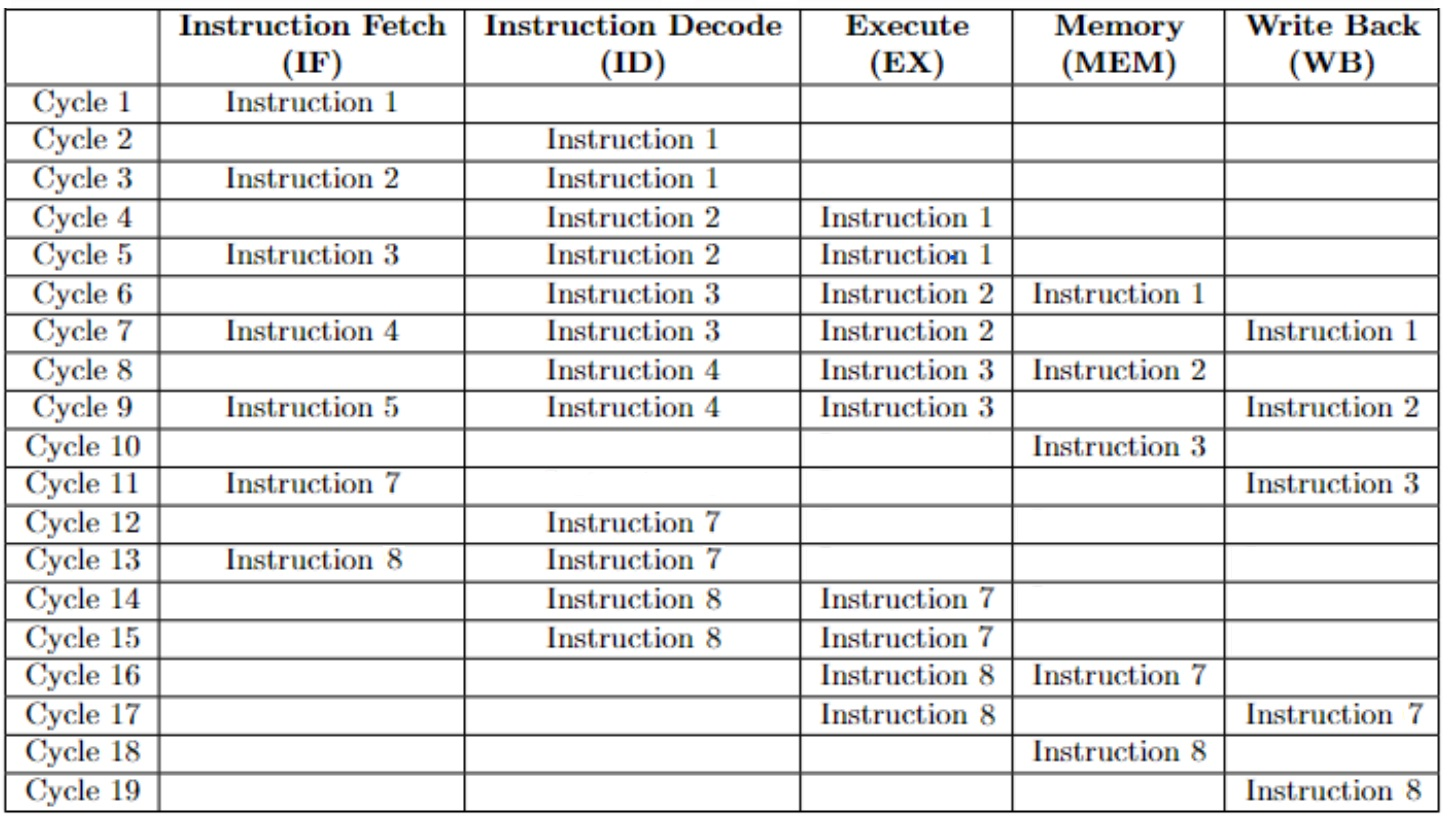
\includegraphics[width=\textwidth]{WhatsApp Image 2024-05-16 at 16.49.55.jpeg}

        \end{figure}

       
    \end{itemize}
    \item \textbf{Termination:}
    \begin{itemize}
        \item Frees allocated memory.
        \item Prints the final state of registers and memory.
    \end{itemize}
\end{enumerate}


\subsection{Pseudo Algorithm}

\textbf{Main Loop:}
\begin{enumerate}
    \item Initialize the MIPS pipeline stages and program counter (PC).
    \item Iterate through pipeline stages in each cycle until all instructions are processed.
    \item Execute each pipeline stage in the following order: Write Back, Memory Access, Execute, Instruction Decode, Instruction Fetch.
    \item Update control signals and data flow between pipeline stages.
    \item Increment the cycle counter to track the progress of execution.
    \item Terminate the loop when all instructions are processed.
\end{enumerate}

\section{Results}

\subsection{Segmentation Faults}

We faced segmentation faults due to illegal memory access, such as dereferencing a null or invalid pointer, or accessing out-of-bounds array indices.

\subsection{Solution}
\begin{itemize}
    \item \textbf{Pointer Initialization}: Ensure all pointers are properly initialized before use. For instance, the pointer arrays like IFID, IDEX, EXMEM, and MEMWB should be allocated enough memory.
    \item \textbf{Bounds Checking}: Implement bounds checking to ensure array indices are within valid range. This is especially crucial when accessing memoryfile and registerFile.
    \item \textbf{Memory Allocation}: Before accessing dynamically allocated memory, check if the memory allocation was successful.

\end{itemize}

\subsection{Uninitialized Variables}

We had some problems with uninitialized variables that led to unpredictable behavior and incorrect results. For instance, when fetchInt, decodeInt, executeInt, or memoryInt were used without being properly initialized, it caused the program to malfunction.

\subsection{Solution}
\begin{itemize}
    \item \textbf{Initialization}: Ensure all variables are properly initialized before use.
    \item \textbf{Default Values}: Set default values for all variables and structures at the beginning of the program.
\end{itemize}

\subsection{Memory Leaks}

We allocated memory dynamically using malloc without freeing it appropriately. If memory is not freed, it led to memory leaks, especially in long-running programs.

\subsection{Solution}
\begin{itemize}
    \item \textbf{Memory Management}: Ensure that all dynamically allocated memory is freed at the end of the program. This is already partly done, but make sure it's comprehensive
\end{itemize}

\subsection{Undefined Behavior in ALU Function}

The ALU function exhibited undefined behavior during operations like multiplication or shifts if inputs were not handled properly.

\subsection{Solution}
\begin{itemize}
    \item\textbf{Sanitize Inputs}: Ensure that inputs to the ALU function from the text file are sanitized and within expected ranges. Implement checks for edge cases, such as large integer values that might cause overflow, and handle negative number inputs from the arithmetic operations.
\end{itemize}

\subsection{Instruction Fetch and Decode Synchronization}

The synchronization between fetch, decode, execute, memory, and writeback stages was not correct, leading to improper instruction execution order.

\subsection{Solution}
\begin{itemize}
    \item \textbf{Pipeline Control}: Ensure that the pipeline stages are correctly synchronized. Implement control logic to manage the pipeline flow, handling hazards and stalls appropriately.
    \item \textbf{Cycle Management}: Verify that the cycle count and stage transitions are accurately implemented.
\end{itemize}

\section{Conclusion}

To sum up, the MIPS pipeline simulation offered insightful knowledge on how a MIPS processor functions and how its pipeline stages behave. The simulation showed where the code needed to be improved, especially in memory management and address manipulation, even if it ran into some problems. By resolving these problems, the simulation can be improved to offer a more realistic depiction of an actual MIPS processor, supporting additional computer architecture research and development.

\end{document}